\documentclass[polish]{inz}

%+Make Index
\usepackage{makeidx}
\makeindex
%-Make Index

\usepackage{polski}
\usepackage[utf8]{inputenc}
\usepackage[OT4]{fontenc}

%+Title
\title{Graficzne interfejsy aplikacji opartych o biblioteki Qt i KDE}
\author{Jan J\k{e}drychowski\\\L{}ukasz Spas}
\date{2012}
\advisor{dr in\.{z}. Igor Wojnicki}
%-Title

\begin{document}
\maketitle

\chapter{Wstęp}

W dzisiejszych czasach coraz bardziej powszechne staje się wykorzystanie przeglądarek do zadań, do których wcześniej używane były duże aplikacje klienckie. Powstają rozwiązania, które starają się oddzielić logikę obliczeniową od warstwy prezentacji, przenosząc jednocześnie tę pierwszą na stronę serwera. Rozwój technologii HTML5 rozszerzającej standard o elementy canvas, websocket, webworkers i inne umożliwia tworzenie aplikacji o możliwościach takich samych jakie niegdyś były dostępne tylko w programach desktopowych. Co więcej gwarantuje międzyplatformowość nie tylko w rozumieniu softwareowym - jedna aplikacja dostępna jest zarówno na komputerach osobistych, tabletach, telefonach i innych urządzeniach wyposażonych w nowoczesną przeglądarkę.

W niektórych rozwiązaniach zastąpienie starych aplikacji desktopowych nowymi aplikacjami webowymi (przeglądarkowymi) jest jednak niemożliwe, czasochłonne lub zbyt kosztowne.

Podczas badań rynku pod kątem aktualnie dostępnych rozwiązań dostrzeżono braki w solucjach umożliwiających zdalną interakcję z pojedynczymi aplikacjami. Większość z rozwiązań dostępnych na rynku wymusza udostępnienie całego pulpitu oraz wymaga od użytkownika końcowego (klienta) posiadania odpowiedniego, nierzadko płatnego oprogramowania (np. TeamViewer, VNC, Citrix i inne). Celem projektu jest stworzenie alternatywy wymagającej od strony klienta jedynie przeglądarki obsługującej HTML5 bez konieczności instalacji jakichkolwiek pluginów (np. Java, Flash).

Głównym wzorcem dla tej pracy jest projekt GTK+ Broadway powstały w 2011 roku oferujący dostęp przez przeglądarkę internetową do aplikacji działających pod kontrolą biblioteki GTK na zdalnym serwerze. Do tej pory nie istniało rozwiązanie oferujące podobną funkcjonalność dla biblioteki Qt i stworzony na potrzeby tej pracy projekt jest pierwszą taką implementacją. Kluczowym czynnikiem wyróżniającym tę pracę na tle innych jest innowacyjny sposób przesyłu danych do wizualizacji okien i ich elementów, który nie opieraja się na transmisji bitmap.

\chapter{Podstawy teoretyczne}
W rodziale tym przedstawione zostaną najważniejsze informacje dotyczące technologii wykorzystanych w projekcie. 

\section{Szczegóły niektórych rozwiązań HTML5}
Text in section ...

\section{Opis biblioteki Qt}
W tym podrozdziale zostaną przedstawione mechanizmy biblioteki Qt wykorzystane przy tworzeniu projektu, o którym stanowi niniejsza praca. 

\subsection{System zdarzeń}
W \emph{Qt} zdarzenia są obiektami dziedziczącymi po klasie \emph{QEvent}, reprezentującymi zajście pewnego zjawiska wewnątrz aplikacji lub będącymi wynikiem oddziaływania z zewnątrz o którym aplikacja powinna wiedzieć. Zdarzenia mogą być przetworzone przez wszystkie obiekty dziedziczące po klasie \emph{QObject}, która dostarcza podstawową strukturę i logikę niezbędną do ich obsługi. 

Kiedy system operacyjny generuje sygnał o zajściu pewnego zdarzenia, \emph{Qt} dokonuje jego konwersji na odpowiedni i platformowo niezależny format. Każde zdarzenie jest następnie przekazywane do \emph{kolejki zdarzeń} odpowiedniego wątku. Kolejka przechowuje i w odpowiednim momencie rozdysponowywuje zdarzenia do odpowiadających im obiektów odbiorców poprzez wywołanie metody \emph{QObject::event()} wewnątrz której następuje decyzja dotycząca dalszego przetwarzania zależna od rodzaju zdarzenia. 

Niektóre zdarzenia, takie jak na przykład \emph{QMouseEvent} czy \emph{QKeyEvent} pochodzą bezpośrednio od systemu operacyjnego. Inne jak na przykład \emph{QTimerEvent} czy \emph{QPaintEvent} pochodzą z innych źródeł, nierzadko z wnętrza samej aplikacji (np. do komunikacji między wątkami). Warto w tym miejscu zaznaczyć, że rysowanie w \emph{Qt} nie jest operacją wywoływaną przez system operacyjny lecz przez samą aplikację oraz rysowanie z wnętrza obsługi zdarzenia \emph{QPaintEvent} jest jedynym sposobem na renderowanie graficznego interfejsu aplikacji. Pociąga to za sobą pewne problemy opisane w dalszej części pracy.

\subsection{System widgetów}


\subsection{System rysowania}
Rysowanie w bibliotece Qt standardowo zostało zaimplementowane dla rysowania na ekranie oraz urządzeniach drukujących wykorzystując natywne API systemu operacyjnego, dla którego dana wersja Qt została skompilowana. Moduł ten jest niejako opakowaniem dla wywołań systemowych ujednolicając jego logikę i umożliwiając pełną przenośność aplikacji. Na rysunku \ref{paintsystem-core} przedstawiony został kaskadowy model systemu rysowania w Qt. Jest to \emph{model trójwarstwowy} i każda z klas ma swoje określone zadanie w całym procesie renderowania. Główną zaletą takiego podejścia jest ujednolicenie przepływu procesu rysowania dla różnych urządzeń wyjściowych oraz umożliwienie łatwego sposobu dla dodawania nowych funkcjonalności.

Klasa \emph{QPainter} udostępnia jednolity interfejs umożliwjający wykonywanie operacji rysowania różnych obiektów takich jak linie, okręgi, prostokąty, obrazy oraz umożliwia zastosowanie różnego rodzaju przekształceń, styli czy transformacji macierzowych. 

Klasa \emph{QPaintDevice} stanoti abstrakcję dla dwuwymiarowej przestrzeni na której obiekty klasy \emph{QPainter} mogą wykonywać operacje rysowania. Udostępnia ona różnego rodzaju informacje dotyczące specyfiki urządzenia wyjściowego, które mogą być wykorzystane np. do optymalizacji procesu rysowania. 

Klasa \emph{QPaintEngine} udostępnia interfejs za pomocą którego obiekty klasy \emph{QPainter} będą mogły wykonywać operacje rysowania na różnego rodzaju urządzeniach wyjściowych. Klasa \emph{QPaintEngine} jest używana wewnątrz klas \emph{QPainter} oraz \emph{QPaintDevice} i jest ukryta przed aplikacjiami dopóki programista nie zechce stworzyć obsługi dla nowego rodzaju urządzenia wyjściowego. W niniejszej pracy taki właśnie scenariusz został wykorzystany.
 
\begin{figure}
  \centering
  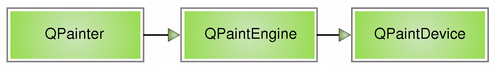
\includegraphics[width=\textwidth,height=!]{img/paintsystem-core.png}
  \caption{Schemat budowy systemu renderowania w bibliotece Qt}
  \label{paintsystem-core}
\end{figure}

\chapter{Określenie problemu i proponowane rozwiązanie}
Text in first chapter ...

\chapter{Implementacja}
Text in first chapter ...

\section{Po stronie serwera}
\label{sec:implementation_server}
Text ...

\section{Po stronie klienta}
Text ...

\section{Napotkane problemy}
Text ...

\chapter{Testy aplikacji}
Text ...

\section{Testy w środowisku lokalnym}
Text ...

\section{Testy w sieci Internet}
Text ...

\chapter{Podsumowanie}
Text ...

%+Make Index
\printindex
%-Make Index

\end{document}